%\documentclass{beamer}
\documentclass[handout]{beamer}
\usepackage[utf8]{inputenc}
\usepackage[T1]{fontenc}
\title{Haptic Pattern Representation\\ Using Music Technologies}
\date[ISPN ’80]{CIM14 Berlin | \texttt{2014-12-04}}
\author[MJC]{Michael Cumming | \texttt{mcumming@ocadu.ca}}

\usetheme{MJC}

\setbeamerfont{page number in head/foot}{}
\setbeamertemplate{footline}[frame number]
\setbeamertemplate{caption}[numbered]

%tikz stuff
\usepackage{tikz}
\usepackage{pgf}
\usetikzlibrary{arrows,shapes,automata}
\usepackage{graphicx}
\usepackage{caption}
\usepackage{subcaption}
\usepackage{float}
\usepackage{natbib}
\bibliographystyle{apalike}
% make bibliography entries smaller
\renewcommand\bibfont{\scriptsize}
% If you have more than one page of references, you want to tell beamer
% to put the continuation section label from the second slide onwards
\setbeamertemplate{frametitle continuation}[from second]

% Now get rid of all the colours
\setbeamercolor*{bibliography entry title}{fg=black}
\setbeamercolor*{bibliography entry author}{fg=black}
\setbeamercolor*{bibliography entry location}{fg=black}
\setbeamercolor*{bibliography entry note}{fg=black}
% and kill the abominable icon
\setbeamertemplate{bibliography item}{}

\begin{document}

\begin{frame}
\titlepage
\end{frame}

\begin{frame}{What is the problem?}
\begin{itemize}
\item Pattern authoring for a non- or quasi-musical device
\begin{itemize}
\item For vibrotactile bands with tactor (vibe motor) arrays
\item Make these patterns convey information and seem `musical'
\end{itemize}
\item Use Standard Musical Notation > Lilypond > MIDI > Arduino 
\item Align these patterns with the configuration of the device
\begin{itemize}
\item For example, if arrays are 2D, design activation patterns to suit
\end{itemize}
\end{itemize}
\bigskip
\centering
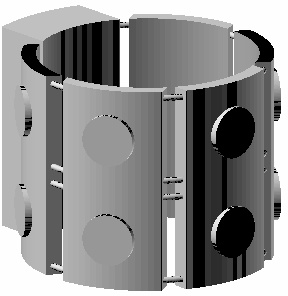
\includegraphics[width=2cm]{graphics/bracelet-02.png}
\hspace{1em}
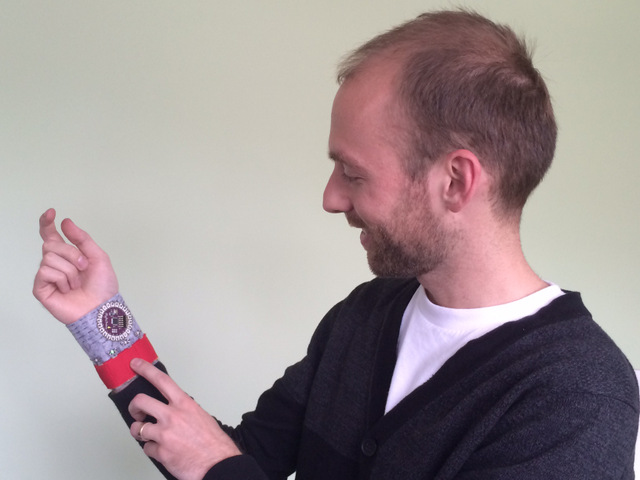
\includegraphics[width=3cm]{graphics/hudsonBand.png} 

\end{frame}

\begin{frame}{Why do this?}
\begin{itemize}
\item Notification and stimulation from such bands could enrich transmedia narratives and gaming experiences
\item Touch, vibration and rhythm are important sensual modalities
\item Authoring rhythmic patterns using music notation is efficient and has a long history
\item Alternatives are not attractive
\end{itemize}
\bigskip
\centering
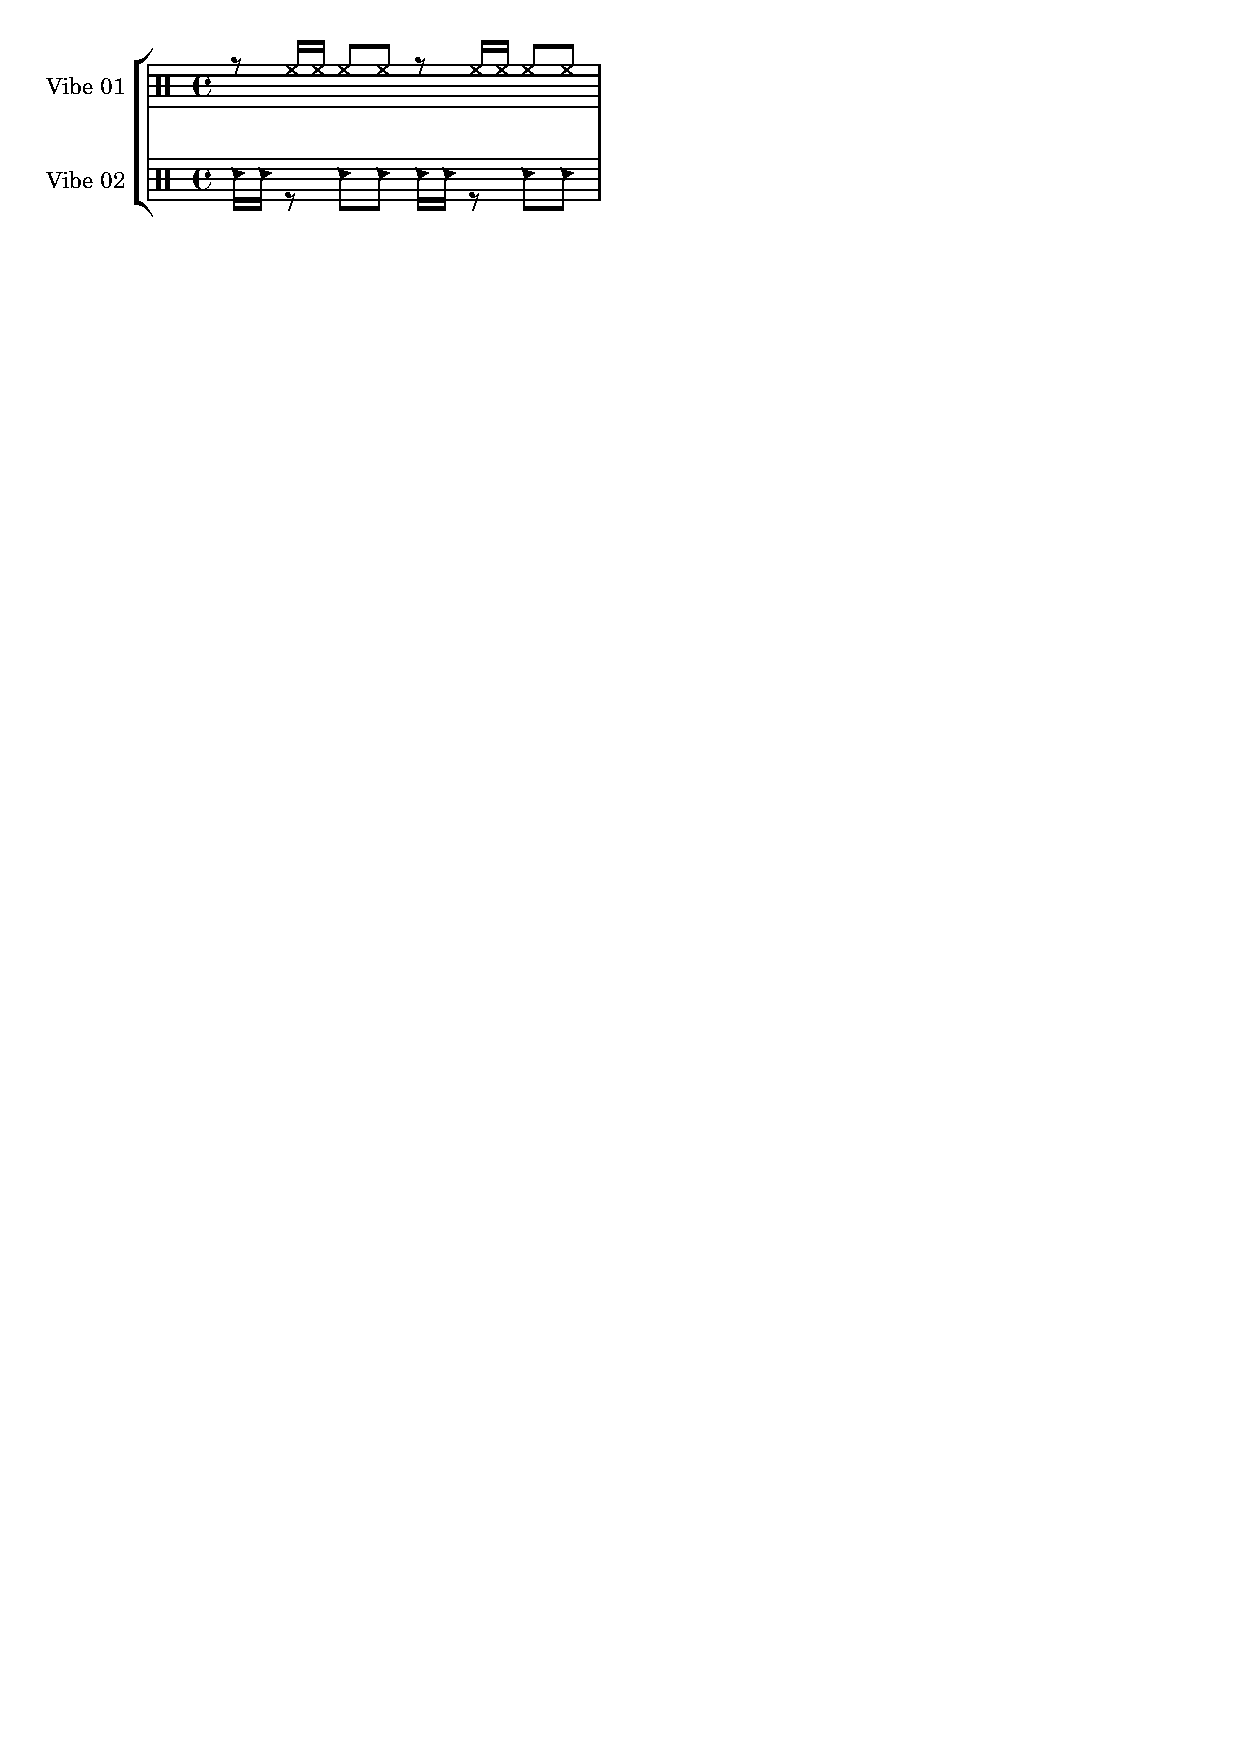
\includegraphics[width=5cm]{graphics/drums1-simple.pdf} 
\end{frame}

\begin{frame}{Findings}

\begin{itemize}

\item Music notation typically occupies 2D: time x (pitch, parts)
\item Vibrotactile bands are also 2D (physical configuration of array)
\item Mapping problem: specify time and pitch, add additional spatial 2D patterns suited to the array
\bigskip
\end{itemize}


\centering
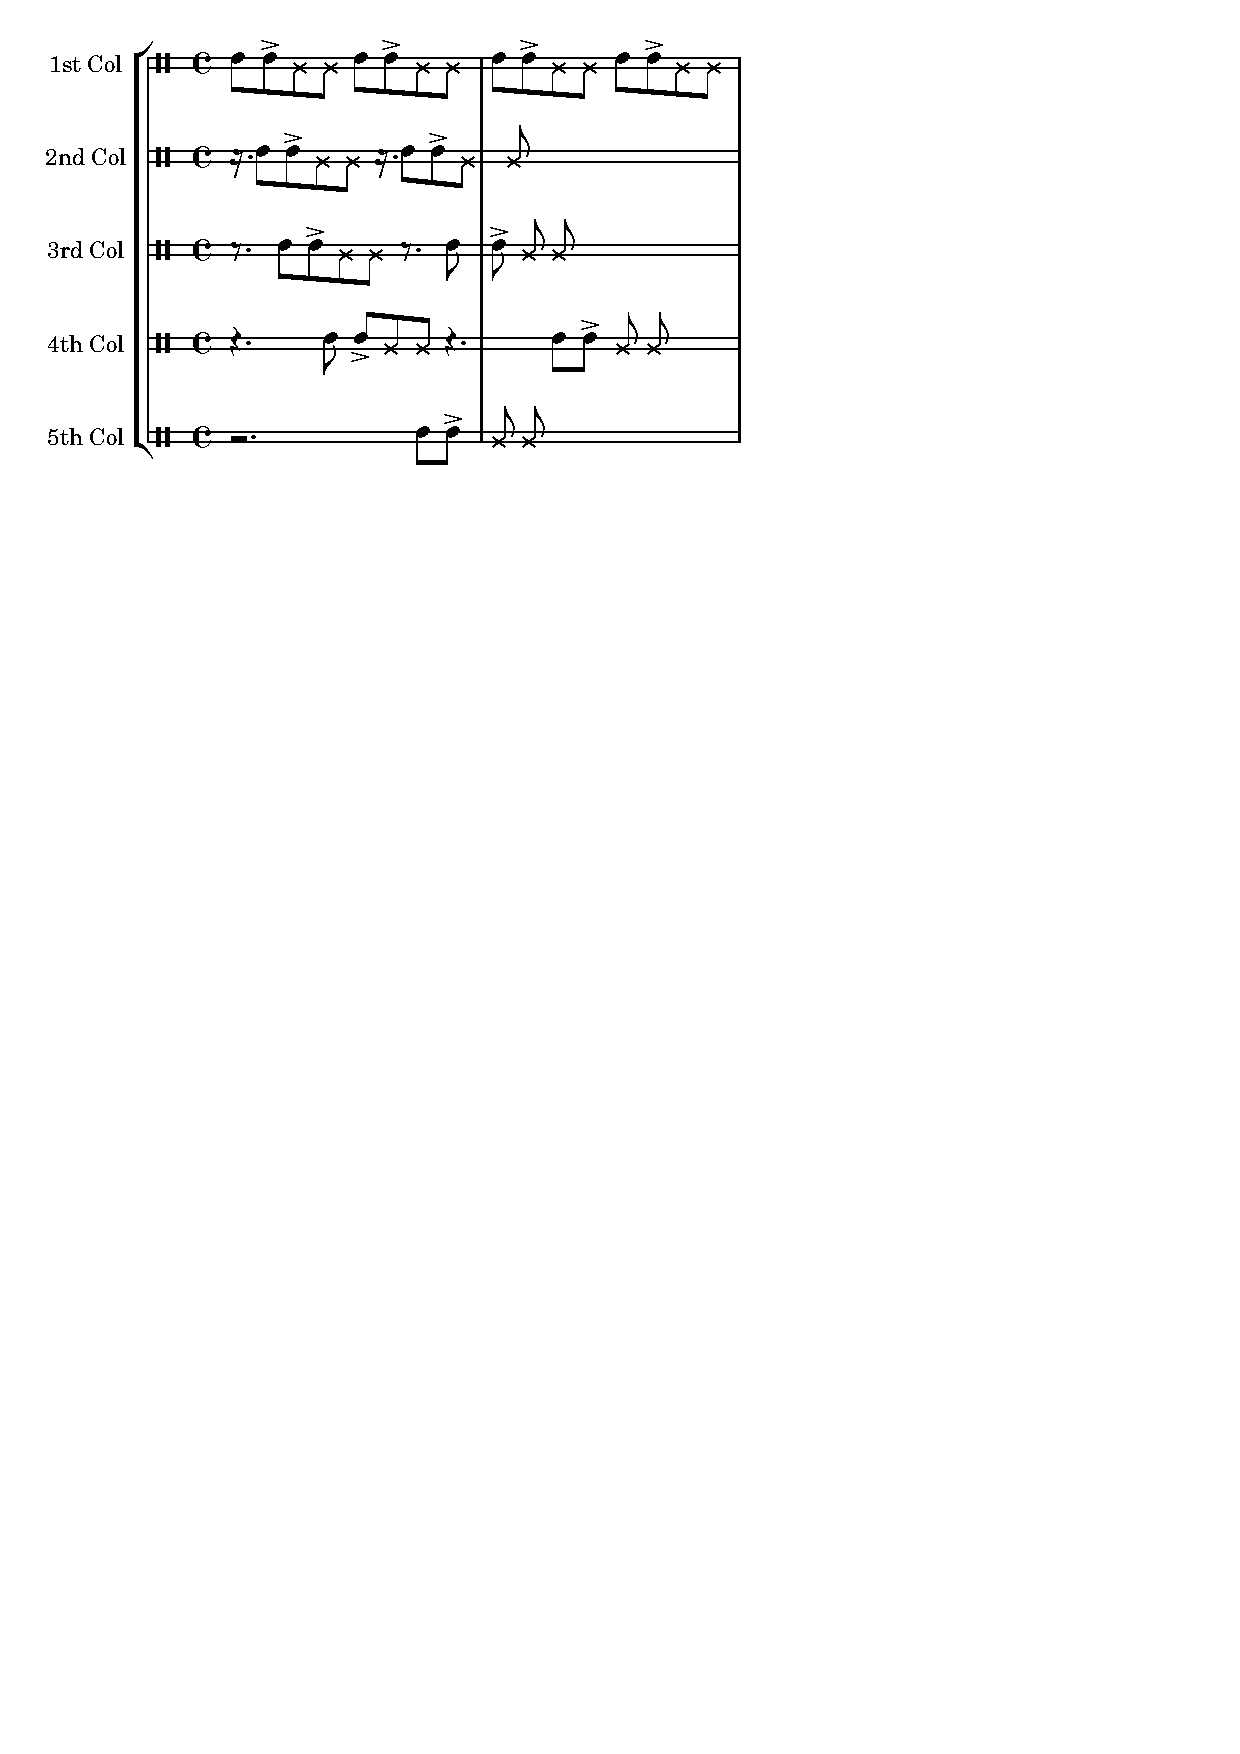
\includegraphics[width=5cm]{graphics/arrowsMoving-5sysx2lines.pdf} 
\bigskip
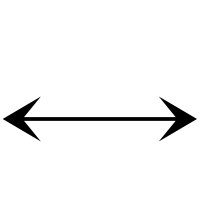
\includegraphics[width=.75cm]{graphics/doubleArrow.png} 
\bigskip
\hspace{1em}
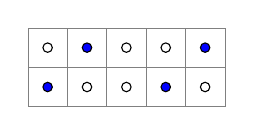
\begin{tikzpicture}[scale=0.5]
%grid
\draw[step=1cm,gray,very thin] (0,0) grid (5,2);
%top row:
\filldraw[fill=white, draw=black] (0.5,1.5) circle (0.12cm);
\filldraw[fill=blue, draw=black] (1.5,1.5) circle (0.12cm);
\filldraw[fill=white, draw=black] (2.5,1.5) circle (0.12cm);
\filldraw[fill=white, draw=black] (3.5,1.5) circle (0.12cm);
\filldraw[fill=blue, draw=black] (4.5,1.5) circle (0.12cm);
%bottom row:
\filldraw[fill=blue, draw=black] (0.5,0.5) circle (0.12cm);
\filldraw[fill=white, draw=black] (1.5,0.5) circle (0.12cm);
\filldraw[fill=white, draw=black] (2.5,0.5) circle (0.12cm);
\filldraw[fill=blue, draw=black] (3.5,0.5) circle (0.12cm);
\filldraw[fill=white, draw=black] (4.5,0.5) circle (0.12cm);
\end{tikzpicture}\\
%\textbf{Device with an array of vibe motors}
\bigskip

\end{frame}


\begin{frame}{Conclusion}
\begin{itemize}
\item Music notation provides a useful, fine-grained graphical representation
\item There are mapping issues with musical notation 
\item Alternatives to music notation seem painful and lack graphical representations
\item Connects the world of music notation to the very young domain of rhythmic wrist wearables

\end{itemize}
\end{frame}

\begin{frame}{Thanks for your attention!}
\hspace{2cm} Michael Cumming\\
\hspace{2cm} OCAD University, Toronto, Canada\\
\bigskip
 \hspace{2cm} \texttt{mcumming@ocadu.ca}
 
 %\bigskip
 %
\includegraphics[width=2cm]{graphics/OCAD_Logo.png}

    
\end{frame}


\end{document}